\FloatBarrier
\section{Results}
\label{sec:results}

We test the \ac{CFT} predictions of Section~\ref{sec:cft:temporal} using simulations of the critical ANNNI-type chain, Eq.~\eqref{eq:annni_H} with $\lambda=1$, quenched from the polarised state $\ket{X+}$. The \ac{NNN} coupling ranges from the integrable point, $p=0$, to $p=0.5$. Extracting the universal data requires a sufficiently long time window, while the computational cost increases rapidly with $p$; we therefore restrict the dynamical calculations to this range.

We follow the two routes introduced in Section~\ref{sec:numerics}: the entropy route, which requires the dominant eigenvectors, and the spectral route, which uses the leading eigenvalues. Both analyses include the integrable Ising point and the non-integrable cases, allowing us to determine whether the conformal signatures persist after introducing the \ac{NNN} interaction. Table~\ref{tab:cp} summarises the resulting universal data.

Unless stated otherwise, the simulations use the second-order \textit{VD2} \ac{MPO} of Section~\ref{sec:mporep}, with time step $\delta t=0.1$, cooling regulator $\beta_0=0.2$ ($N_\beta=4$), and maximum temporal bond dimension $\chi=64$. We convert the spectral measurements into universal quantities using the independently determined sound velocities $v_\infty(p)$ from Section~\ref{sec:annni:velocity}. Appendix~\ref{app:errors} gives the fitting conventions and numerical controls.

\begin{table}[!htbp]
    \centering
    \begin{tabular}{lc|ccc|cc}
        \hline
              &            & \multicolumn{3}{c|}{spectral route} & \multicolumn{2}{c}{entropy route} \\
        $p$   & $v_\infty$ & window   & $c$    & $x_1$   & window        & $c$    \\
        \hline
        $0$   & $2.000$    & $T\le24$ & $0.45$ & $0.498$ & $8\le T\le24$ & $0.50$ \\
        $0.1$ & $2.670$    & $T\le17$ & $0.47$ & $0.497$ & $4\le T\le13$ & $0.50$ \\
        $0.3$ & $3.967$    & $T\le10$ & $0.49$ & $0.493$ & $2\le T\le9$  & $0.53$ \\
        $0.5$ & $5.212$    & $T\le6$  & $0.53$ & $0.487$ & $2\le T\le5$  & $0.58$ \\
        \hline
    \end{tabular}
    \caption{\textbf{Universal data as a function of the \ac{NNN} coupling.} The spectral central charge is obtained from the phase curvature of $\mu_0$ through Eq.~\eqref{eq:cft:eq3}, while $x_1$ follows from the first phase gap through Eq.~\eqref{eq:cft:eq4}. The entropy-route central charge is extracted from the extrapolated plateau of Section~\ref{sec:results:wall}, using seed ensembles of independent single-vector runs. Each route has its own fitting window, listed beside its result. Sensitivity to that window dominates the uncertainty of the entropy values and increases as the available ladders shorten. The values at $p=0.3$ and $p=0.5$ are therefore indicative rather than precise. Appendix~\ref{app:errors} gives the fitting conventions and controls.}
    \label{tab:cp}
\end{table}

\subsection{The entropy route}
\label{sec:results:validation}
\label{sec:results:wall}

At the integrable point, the generalised temporal entropy of Eq.~\eqref{eq:s2gen} follows the conformal prediction previously established for the Loschmidt echo of the critical Ising chain~\cite{carignano_tagliacozzo2025}. This behaviour persists after introducing the \ac{NNN} interaction. Figure~\ref{fig:domes} shows the R\'enyi-2 profiles at $p=0.1$: the real part follows the chord dependence of Eq.~\eqref{eq:cft:chord}, while the imaginary part develops a plateau across the interior of the strip. In this comparison, we fix $c=\tfrac12$ and fit only the non-universal constant $s_0$. Appendix~\ref{app:highp} presents the corresponding profiles at the other couplings.

\begin{figure}[htbp]
    \centering
    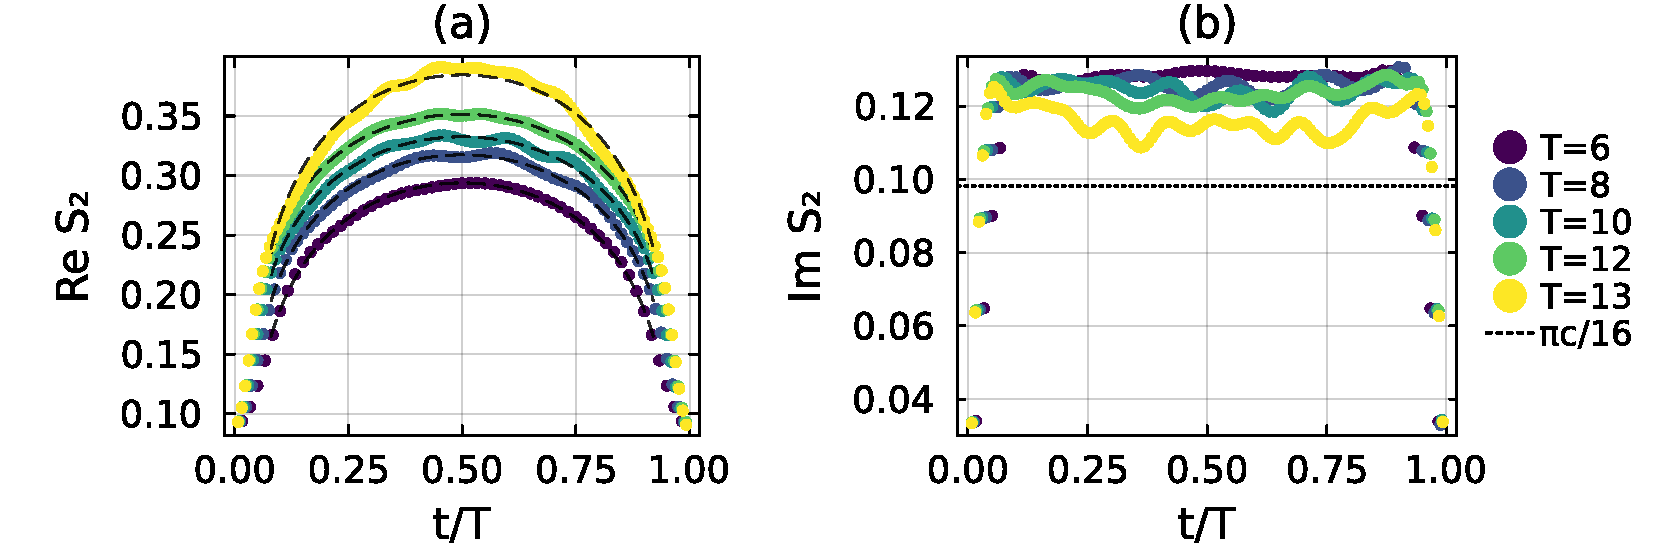
\includegraphics[width=\textwidth]{imgs/res_domes.pdf}
    \caption{\textbf{Generalised temporal entropy at $p=0.1$.} Each colour denotes one evolution time. (a) Real part as a function of $t/T$; the dashed curves show the conformal profile of Eq.~\eqref{eq:cft:chord} with $c=\tfrac12$. (b) Imaginary part, which forms an approximately constant plateau in the interior of the strip. The plateau lies above the asymptotic value $\pi c/16$ (dotted line) and approaches it as $T$ increases.}
    \label{fig:domes}
\end{figure}

At all simulated times, the measured plateau lies above the asymptotic value $\pi c/16$, consistent with the finite-time correction introduced in Section~\ref{sec:cft:temporal}~\cite{boucomas2026}. Determining the asymptote therefore requires an extrapolation over several evolution times, whose reliability depends on the length of the available sequence. Within a short window, the predicted decay and a constant offset describe the data comparably well but extrapolate to different limits, leaving the asymptotic value poorly constrained. Appendix~\ref{app:errors} compares four candidate extrapolation forms and identifies the times at which their predictions separate.

This window dependence accounts for the entropy-route values in Table~\ref{tab:cp}, which are fitted rather than fixed to $c=\tfrac12$ as in Figure~\ref{fig:domes}. The longer ladders at $p=0$ and $p=0.1$ recover the Ising value. The shorter ladders at $p=0.3$ and $p=0.5$ instead yield larger values, consistent with the direction of the finite-time correction but not yet converged. The truncation control at the integrable point quantifies the corresponding shift when the fit is restricted to a short window.

The accessible time window shortens as $p$ increases, leaving fewer points with which to constrain the decay. We terminate each window when the ensembles described in Section~\ref{sec:reach} cease to produce physical entropy profiles reliably. The fraction of unphysical runs increases with $T$ at every coupling, and almost no runs remain usable beyond the windows reported in Table~\ref{tab:cp}. At $p=0.5$ and $T=6$, none of the runs produces a physical profile (Appendix~\ref{app:failures}).


\subsection{The spectral route}
\label{sec:results:spectral}


We compute the leading spectrum over the time windows listed in Table~\ref{tab:cp}. As shown in Figure~\ref{fig:circle}, the trajectory of $\mu_0$ remains close to a circle whose radius depends on the coupling: its phase winds with $T$, while its modulus varies by roughly $1\%$ or less over each ladder. This approximately constant modulus is the signature of emergent dual unitarity discussed in Section~\ref{sec:cft:temporal}. The phase advance also provides a criterion for terminating each ladder. It is nearly constant along the physical branch, and a persistent departure from this behaviour indicates that the branch is no longer resolved.



We extract the central charge from the phase curvature using Eq.~\eqref{eq:cft:eq3} and the fitting conventions of Appendix~\ref{app:errors}. The resulting fits are shown in Figure~\ref{fig:eq3}.

\begin{figure}[!htb]
    \centering
    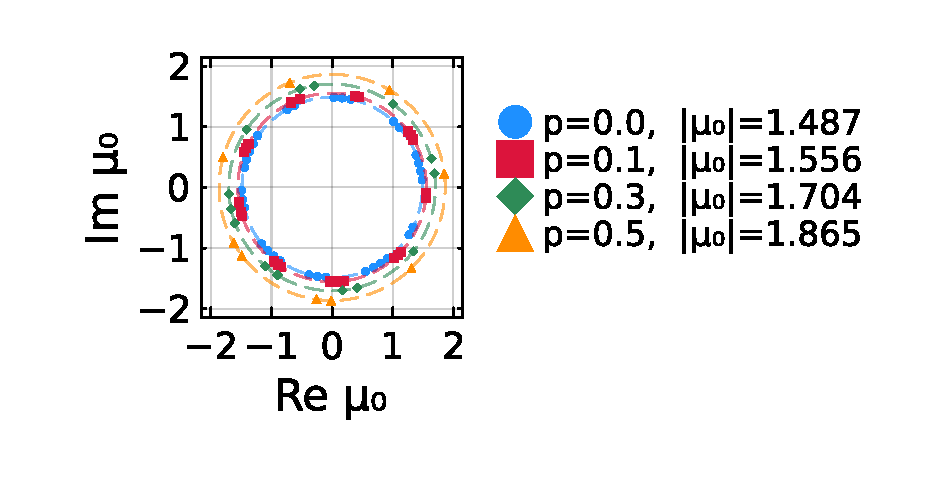
\includegraphics[width=0.70\textwidth]{imgs/res_circle.pdf}
    \caption{\textbf{Trajectory of the leading eigenvalue.} For each coupling, the dashed circle has the mean modulus of the corresponding ladder and is labelled by that value. The phase winds with $T$, while the modulus remains approximately constant.}
    \label{fig:circle}
\end{figure}

The spectral estimates in Table~\ref{tab:cp} remain within approximately $10\%$ of the Ising value at every coupling and are consistent with $c=\tfrac12$ within the resolution of the fits. The equilibrium chord analysis of Section~\ref{sec:annni:equilibrium} gives comparable estimates over the same coupling range. This agreement provides an independent comparison between universal data extracted from the ground state and from real-time dynamics.

The two routes deviate from the conformal value for different reasons. In the entropy route, the plateau approaches $\pi c/16$ from above, and its asymptotic value must be obtained through the extrapolation described in Section~\ref{sec:results:wall}. At the integrable point, the spectral estimate is instead biased downwards to approximately $0.45$ by two finite-parameter corrections quantified separately in Appendix~\ref{app:x1}. First, Eq.~\eqref{eq:cft:eq3} gives only the leading term in an expansion in $1/T$; including the next-order term raises the fitted coefficient from $90\%$ to $97\%$ of its predicted value. Second, the regulator contributes through $\beta_0/T$. The fitted coefficient decreases linearly with $\beta_0$ and extrapolates to the predicted value as $\beta_0\to0$. That limit is an extrapolation rather than an accessible setting, since without the cooling interval the initial state is a bare product state and not a conformal boundary state (Section~\ref{sec:cft:boundary}), so the strip would have no well-defined conformal edge from which to read the universal data, while the production value $\beta_0=0.2$ produces a downward shift of approximately $10\%$. The observed discrepancy is therefore consistent with controlled finite-time and finite-regulator effects.

The sound velocity affects the spectral analysis in two ways. Equation~\eqref{eq:cft:eq4} gives phase gaps proportional to $1/(vT)$, so a larger velocity compresses the tower at fixed evolution time and requires finer phase resolution. The conversion from the fitted curvature to the central charge also carries a factor of the velocity, since $c=24\,v\,|C|/\pi$, so a fixed uncertainty in $C$ produces an uncertainty in $c$ that grows with $v$. Both effects reduce the spectral resolution at stronger coupling.

The windows of Table~\ref{tab:cp} also shorten as $p$ increases, and we do not attribute this to a single cause. Both effects above contribute, and the conditioning of the left and right states is measured to worsen sharply with the coupling for reasons that remain unresolved (Appendix~\ref{app:conditioning}). The present measurements do not separate these contributions.

\begin{figure}[!tbp]
    \centering
    
\includegraphics[width=0.8\textwidth]{imgs/res_eq3.pdf}
    \caption{\textbf{Central charge from the phase of the leading eigenvalue.} Fits of Eq.~\eqref{eq:cft:eq3} to $\mathrm{Im}\,\lambda_0/T$ at each coupling. The fitted constant $a_0$ is subtracted to display only the time-dependent contribution, whose curvature determines the central charge reported in each legend.}
    \label{fig:eq3}
\end{figure}

\begin{figure}[!tbp]
    \centering
    
\includegraphics[width=0.8\textwidth]{imgs/res_tower.pdf}
    \caption{\textbf{Boundary dimensions as a function of evolution time.} The seven leading dimensions at each coupling are obtained from the phase gaps through Eq.~\eqref{eq:cft:eq4}, ordered by increasing phase distance from $\mu_0$, and resolved using $k=8$. The dashed lines mark the predicted values $\tfrac12$, $\tfrac32$, $2$, $\tfrac52$, $3$, $\tfrac72$, and $4$. These values belong to the two towers selected by the free boundary condition: the identity tower contains the integers, while the energy tower contains the half-integers.}
    \label{fig:tower}
\end{figure}

The Ising boundary spectrum persists after introducing the \ac{NNN} interaction. Figure~\ref{fig:tower} shows the seven leading dimensions resolved with $k=8$. The leading dimension, reported in Table~\ref{tab:cp}, remains within $3\%$ of the predicted value $\tfrac12$ at every coupling.

The first five dimensions remain close to their predicted values throughout the coupling range. The sixth and seventh show a systematic upward drift, reaching $4.23$ and $4.65$ at $p=0.5$, compared with the predicted values $\tfrac72$ and $4$. They are obtained from the highest states retained by the block and are therefore the least converged, as quantified directly in Appendix~\ref{app:blockpm:schur}. Their phase gaps are also the most difficult to resolve as the spectrum becomes increasingly compressed.
